\section{Prototypical service mesh implementation}

The following chapter describes our concept of our prototypical service mesh implementation and its outcome. In order to also practically work out the differences between service meshes and a traditional microservice operation, we will initially run our application using only Kubernetes, and then later set up a service mesh.

\begin{figure*}
    \centering
    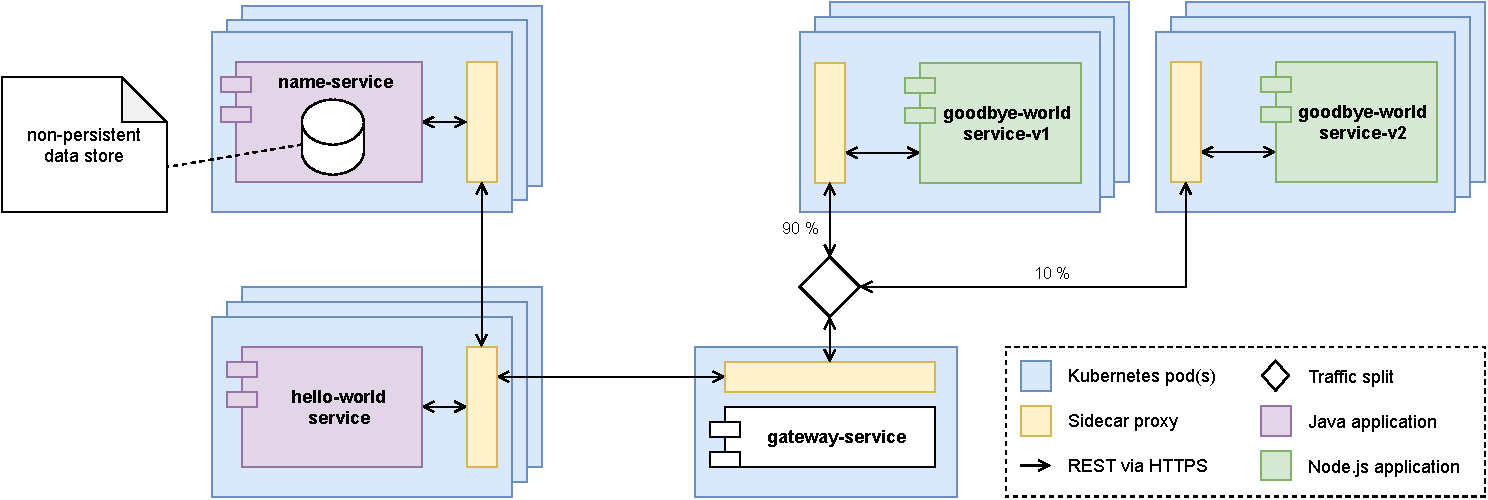
\includegraphics[width=\textwidth]{img/diagram-draft.pdf}
    \caption{Architecture overview of the PoC application}
    \label{fig:poc-overview}
\end{figure*}

\subsection{Services}

Our basic idea is to implement three simple microservice applications that communicate via REST. To prove technology independence, one service is written in Node.js, while the other two services are written in Python. Another requirement to meet is that the services have to be as simple as possible. Furthermore, the functionality of the services is intended to be as follows:

\begin{itemize}
\item \textsc{name-service}: Provides endpoint to retrieve a collection of names. It stores the names in a file or a simple array list.
\item \textsc{goodbye-world-service}: Provides endpoint to retrieve a message ``Goodbye, World!"
\item \textsc{hello-world-service}: Contacts the \textsc{name-service} and provides an endpoint that returns a ``Hello, \{name\}" message for each name object from name service.
\end{itemize}

Since Linkerd does not provide an own ingress controller (see chapter \ref{linkerd}), we use an external ingress controller named \textsc{traefik}.

\subsection{Showcases}

Our prototypical implementation aims to provide answers to the following five challenges of running and maintaining microservices.

\subsubsection{Encryption}

By using a service mesh, it should be shown that an encryption policy can be easily applied or removed.

\subsubsection{Canary Deployment}

To provide an example showcase for canary deployment, we implemented two versions of \textsc{goodbye-world-service} which differ minimally by the returned string. The mesh is tasked with redirecting traffic so that 90\% of all requests are made to version 1 and 10\% of requests are made to version 2.

\subsubsection{Access Policies}

Another restriction is that the \textsc{name-service} is only accessible from the \textsc{hello-world-service}. Access restriction should not be a task of the actual \textsc{name-service} application. We want to show that access to services is easily managable via YAML resources.

\subsubsection{Central monitoring and logging}
The proof of concept should show that services in a microservice landscape can be monitored and managed centrally using the service mesh.

\subsection{Setup of Linkerd}

The following sequence of bash commands shows the \textsc{Linkerd} installation process and the application of the service mesh to the \textsc{Kubernetes} cluster \cite{linkerd-get-started}:
\begin{lstlisting}[language=bash,caption={Setup of \textsc{Linkerd}}, label={lst:linkerd-setup}]
#!/bin/bash
curl -sL https://run.linkerd.io/install \
	| sh
export PATH=$PATH:$HOME/.linkerd2/bin
echo "export PATH=$PATH:$HOME/.linkerd2/bin" \
	>> ~/.bashrc
linkerd install | kubectl apply -f -
\end{lstlisting}

\subsection{Resource definition for applications}

\subsection{Policy application}